\documentclass[12pt,letterpaper]{article}
\usepackage[utf8]{inputenc}
\usepackage[T1]{fontenc}
\usepackage[spanish,es-nodecimaldot]{babel}
\usepackage[margin=1in,headheight=15pt]{geometry}
\usepackage{newtxtext,newtxmath,setspace,fancyhdr,graphicx,booktabs,caption,float,xurl,hyperref,titlesec,listings}
\hypersetup{hidelinks,pdftitle={Verificación facial con una red siamesa},pdfauthor={Karen Sofía Delgado Calderon}}
\urlstyle{same}
\doublespacing
\setlength{\parindent}{0.5in}
\pagestyle{fancy}\fancyhf{}\rhead{\thepage}\renewcommand{\headrulewidth}{0pt}
\titleformat{\section}{\normalfont\normalsize\bfseries\centering}{}{0pt}{}
\captionsetup{labelsep=newline,labelfont=bf,textfont=it,justification=raggedright,singlelinecheck=false}
\addto\captionsspanish{\renewcommand{\tablename}{Tabla}}
\newcommand{\refapa}[1]{\par\noindent\hangindent=0.5in\hangafter=1 #1\par}
\newcommand{\tituloinforme}{Verificación facial con una red siamesa y pocas referencias}
\begin{document}
\begin{titlepage}\thispagestyle{fancy}
\begin{center}\vspace*{1.35in}
\textbf{\tituloinforme}\par\vspace{\baselineskip}
Karen Sofía Delgado Calderon\par
Universidad de Cundinamarca\par
Especialización en Inteligencia Artificial\par
Deep Learning -- Conceptos\par
R2-A1-S10 Redes Neuronales V\par
5 de noviembre de 2026
\end{center}
\end{titlepage}
\setcounter{page}{2}
\begin{center}\textbf{\tituloinforme}\end{center}

Una fotografía de referencia puede ser insuficiente cuando cambian la pose, la iluminación y la expresión. Esta práctica mide cuánto aporta una red siamesa frente a una comparación directa de píxeles y cuánto cambia el resultado al pasar de una a cinco referencias por identidad. La prueba usa fotografías públicas de \textit{Labeled Faces in the Wild} (LFW) e identidades que quedaron fuera del ajuste. Con cinco referencias, la red acierta el 43,29\% de las consultas, frente al 33,54\% de la línea base.

\section{Corpus y preprocesamiento}
LFW reúne fotografías faciales públicas en condiciones variadas (Huang et al., 2007). Se usó la variante alineada \textit{funneled} distribuida por el cargador de scikit-learn, con recorte facial y conversión a grises (Scikit-learn developers, s. f.). Al pedir al menos 20 imágenes por identidad se obtuvieron 3.023 recortes de $62\times47$ píxeles. Para reducir la diferencia de peso entre identidades, se seleccionaron entre 20 y 24 recortes por clase. Antes de seleccionar se verificaron copias exactas mediante SHA-256 sobre el recorte cargado.

Cada recorte se redujo a $40\times30$ por área, conservando aproximadamente su proporción. Se restó su intensidad media y se dividió por su desviación estándar. Esta operación reduce diferencias globales de brillo y contraste y conserva la estructura espacial de la cara. Puede perderse detalle al reducir la resolución. Las imágenes ya llegan alineadas y recortadas, de modo que esta práctica empieza después de la detección y el alineamiento originales.

\begin{table}[H]
\caption{Inventario por fase del experimento}\label{tab:particiones}
\centering
\begin{tabular}{lrrl}\toprule
Fase & Identidades & Fotos & Uso\\\midrule
Ajuste & 40 & 929 & Aprender pesos\\
Calibración & 10 & 234 & Elegir umbrales\\
Prueba & 12 & 280 & Medir desempeño\\\midrule
Total & 62 & 1.443 & \\\bottomrule
\end{tabular}
\par\vspace{4pt}\raggedright\footnotesize\textit{Nota.} La partición por identidad se generó con semilla 487. Una identidad se asigna a una sola fase. Los recuentos provienen de \texttt{resumen\_lfw.json}.
\end{table}

La Tabla~\ref{tab:particiones} separa por completo las identidades de cada fase. Así, la prueba mide transferencia a personas ausentes durante el ajuste y la calibración. Los archivos de entrega contienen el código de descarga, resultados agregados y la fuente del corpus. La procedencia pública se documenta con la referencia al conjunto de investigación.

\section{Codificador y función de costo}
Las ramas de la red siamesa comparten un mismo codificador. Tres capas convolucionales con filtros de $3\times3$ producen 16, 32 y 48 canales, con ReLU y dos reducciones espaciales mediante máximo. El promedio adaptativo entrega un mapa de $48\times4\times3$, que una capa lineal proyecta a 32 dimensiones. La normalización de norma dos deja cada vector en una esfera unitaria. El modelo tiene 37.136 parámetros entrenables.

El entrenamiento reúne un ancla $a$, otra toma $p$ de la misma identidad y una toma $n$ de una identidad distinta. La pérdida penaliza tríos donde la distancia positiva queda demasiado cerca de la negativa, siguiendo el principio de FaceNet (Schroff et al., 2015). Con $d$ como distancia euclidiana entre representaciones y margen 0,30, la pérdida por trío es
\[
  L(a,p,n)=\max\{0,\ d(a,p)-d(a,n)+0{,}30\}.
\]
Se usó Adam con tasa 0,001 durante 24 épocas, con ocho lotes de 48 tríos por época. Cada positivo es una captura distinta del ancla. Las tres entradas pasan por los mismos pesos y la pérdida media del lote dirige el ajuste. El código completo se incluye en el apéndice.

\section{Protocolo de reconocimiento y verificación}
Cada episodio reserva cinco tomas por identidad para la galería y diez tomas distintas como consultas. En \textit{one-shot} se emplea la primera toma de la galería. En \textit{few-shot} se forma un prototipo con el promedio normalizado de las cinco representaciones, siguiendo la idea de prototipos de Snell et al. (2017). La línea base aplica la misma regla de galería a los 1.200 píxeles normalizados. Ambas representaciones reciben exactamente las mismas consultas.

El reconocimiento cerrado elige el prototipo más cercano entre las identidades de prueba. La verificación aplica un umbral de distancia a cada pareja consulta--prototipo. Se calibró un umbral por método y número de referencias con diez episodios, maximizando la diferencia entre la tasa de verdaderas aceptaciones y la tasa de falsas aceptaciones. Luego se congeló el umbral y se evaluaron veinte episodios sobre las 12 identidades reservadas.

En verificación, FAR divide las falsas aceptaciones por las comparaciones entre identidades distintas. FRR divide los falsos rechazos por las comparaciones de la misma identidad. El área bajo la curva ROC (AUC) resume el orden de distancias al variar el umbral. \textit{Zero-shot} requiere asignar una clase sin fotos de referencia usando información auxiliar. Aquí las identidades de prueba son nuevas para el codificador, pero cuentan con una galería y se evalúan como \textit{one-shot} y \textit{few-shot}.

\section{Resultados}
La pérdida media pasó de 0,2503 a 0,1001. La Figura~\ref{fig:resultados} muestra las fluctuaciones durante el ajuste y la diferencia entre los dos métodos en prueba. Con una referencia la red supera a los píxeles por 8,25 puntos porcentuales. Con cinco, la diferencia es de 9,75 puntos. La exactitud de la red sube 14,17 puntos al ampliar la galería.

\begin{figure}[H]
\caption{Pérdida de entrenamiento y exactitud en identidades reservadas}\label{fig:resultados}
\centering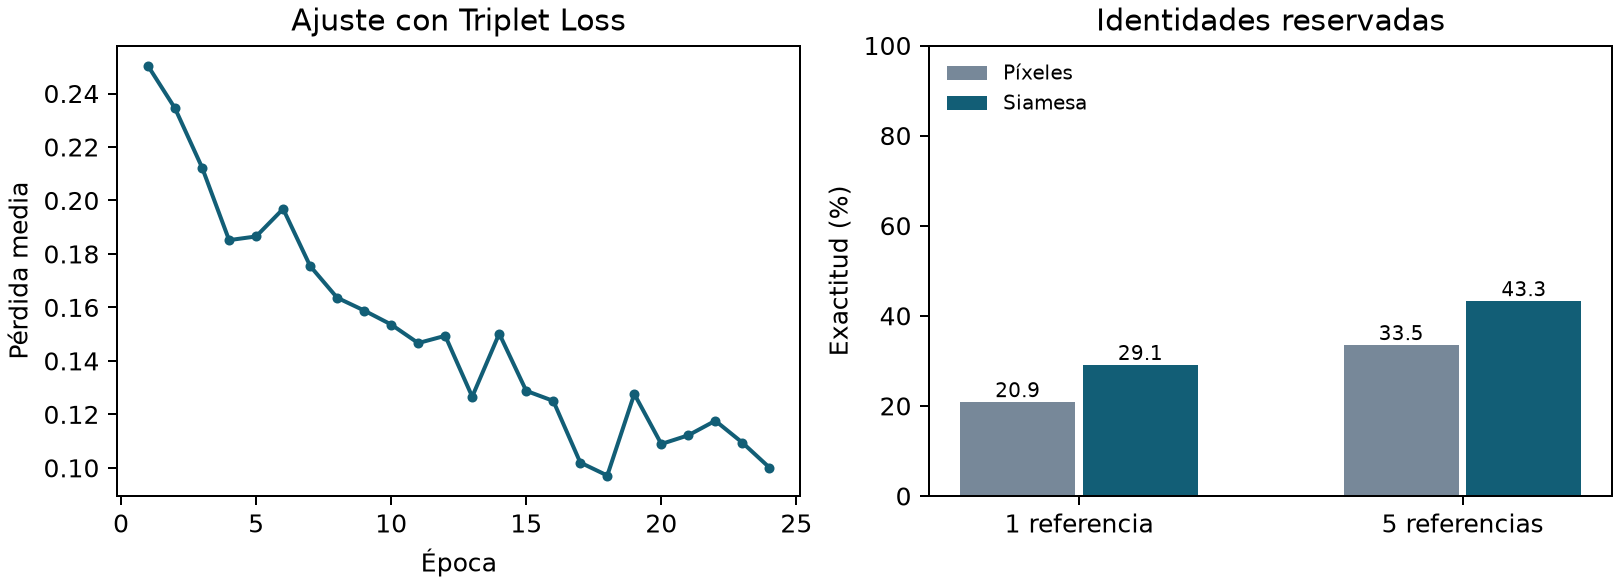
\includegraphics[width=\textwidth]{resultados_lfw.png}
\par\raggedright\footnotesize\textit{Nota.} La curva muestra la media de ocho lotes por época. Las barras resumen 20 episodios por condición. Elaboración propia a partir de \texttt{resumen\_lfw.json}.
\end{figure}

\begin{table}[H]
\caption{Desempeño en reconocimiento cerrado y verificación}\label{tab:resultados}
\centering\small
\begin{tabular}{lrrrrrr}\toprule
Método & $k$ & Aciertos & Exactitud & FAR & FRR & AUC\\\midrule
Píxeles & 1 & 501 & 20,88\% & 45,71\% & 40,75\% & 0,604\\
Píxeles & 5 & 805 & 33,54\% & 46,57\% & 29,50\% & 0,679\\
Siamesa & 1 & 699 & 29,12\% & 31,43\% & 31,37\% & 0,753\\
Siamesa & 5 & 1.039 & 43,29\% & 24,32\% & 23,92\% & 0,841\\\bottomrule
\end{tabular}
\par\vspace{4pt}\raggedright\footnotesize\textit{Nota.} $k$ indica referencias por identidad. Cada fila reúne 2.400 consultas y 26.400 comparaciones entre identidades distintas. Las fotos pueden reutilizarse entre episodios. Fuente: \texttt{resumen\_lfw.json}.
\end{table}

La Tabla~\ref{tab:resultados} muestra que el modelo separa mejor las parejas en ambas configuraciones. Con cinco referencias y umbral 0,7126, hubo 6.421 falsas aceptaciones de 26.400 comparaciones negativas y 574 falsos rechazos de 2.400 positivas. Con una referencia el umbral fue 0,8469. La reducción de ambos errores en este experimento favorece el uso de varias tomas, aunque la comparación conserva un margen de error considerable.

\section{Reproducción y conclusiones}
El \href{https://github.com/sofiadelcal/karen-calidad-imagenes-publicas-s10}{repositorio GitHub de Karen} reúne el código, las dependencias y los resultados. El \href{https://colab.research.google.com/github/sofiadelcal/karen-calidad-imagenes-publicas-s10/blob/main/Karen_Siamesa_LFW.ipynb}{cuaderno en Google Colab} descarga LFW mediante scikit-learn. Para repetir la práctica en CPU, elija \textit{Entorno de ejecución} y \textit{Ejecutar todo}.

La Tabla~\ref{tab:resultados} corresponde a la corrida local. En Colab se obtuvieron 723 y 1.087 aciertos, equivalentes a 30,12\% y 45,29\% con una y cinco referencias. La línea base obtuvo los mismos recuentos en ambos entornos. La Figura~\ref{fig:colab} muestra la finalización del cuaderno y las métricas de esa segunda corrida.

\begin{figure}[H]
\caption{Ejecución del experimento LFW en Google Colab}\label{fig:colab}
\centering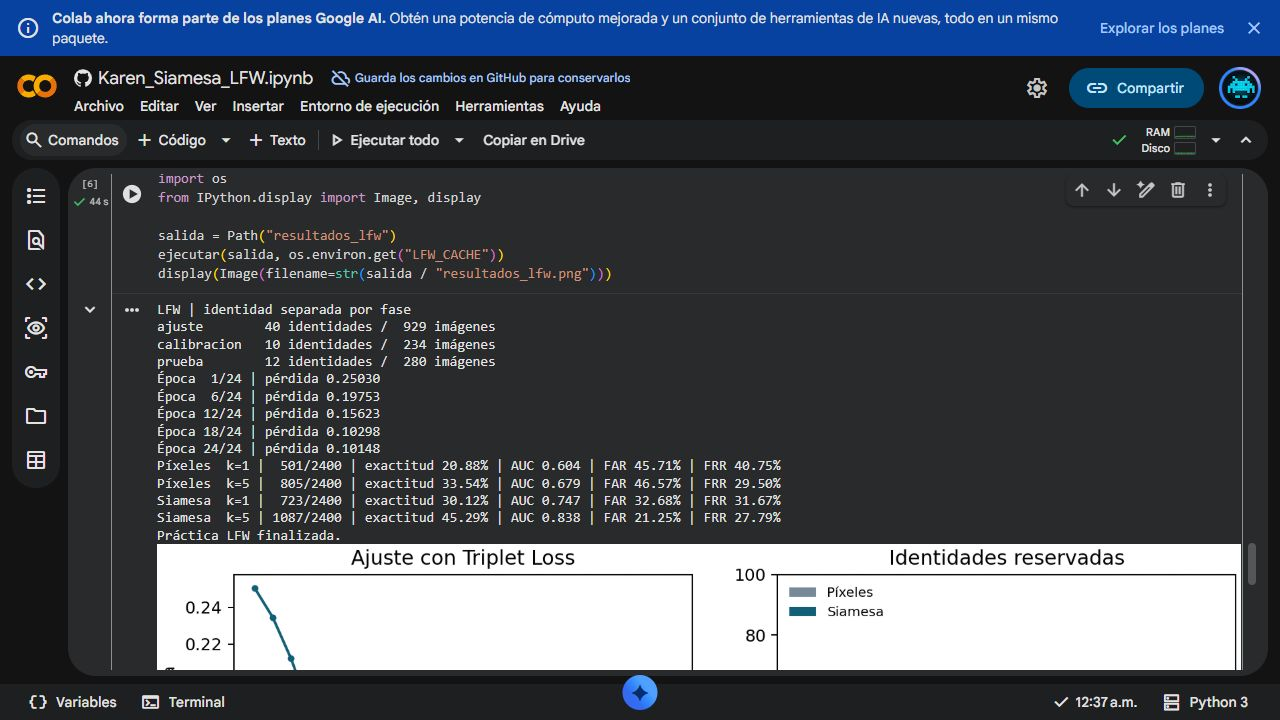
\includegraphics[width=\textwidth,trim=0 170bp 0 0,clip]{evidencia_colab_lfw.png}
\par\raggedright\footnotesize\textit{Nota.} Captura propia del 5 de noviembre de 2026. El entorno de Colab completó las seis celdas de código. Los valores de la red varían entre la corrida de Colab y la local.
\end{figure}

La red mejoró la exactitud cerrada y el AUC frente a la línea base, con el mejor resultado al usar cinco referencias. La muestra favorece identidades con muchas fotos. Los episodios reutilizan imágenes y se evaluó una sola partición, por lo que las cifras describen este protocolo en LFW.

\clearpage
\section{Referencias}
\refapa{Huang, G. B., Ramesh, M., Berg, T., \& Learned-Miller, E. (2007). \textit{Labeled Faces in the Wild: A database for studying face recognition in unconstrained environments} (Technical Report No. 07-49). University of Massachusetts Amherst. \url{https://people.cs.umass.edu/~elm/papers/lfw.pdf}}
\refapa{Schroff, F., Kalenichenko, D., \& Philbin, J. (2015). FaceNet: A unified embedding for face recognition and clustering. En \textit{2015 IEEE Conference on Computer Vision and Pattern Recognition} (pp. 815--823). IEEE. \url{https://doi.org/10.1109/CVPR.2015.7298682}}
\refapa{Scikit-learn developers. (s. f.). \textit{fetch\_lfw\_people}. Scikit-learn. \url{https://scikit-learn.org/stable/modules/generated/sklearn.datasets.fetch_lfw_people.html}}
\refapa{Snell, J., Swersky, K., \& Zemel, R. S. (2017). Prototypical networks for few-shot learning. \textit{Advances in Neural Information Processing Systems, 30}. \url{https://papers.nips.cc/paper_files/paper/2017/hash/cb8da6767461f2812ae4290eac7cbc42-Abstract.html}}

\clearpage
\section{Apéndice}
\begin{center}\textbf{Código de la práctica facial}\end{center}
\begingroup\singlespacing
\lstinputlisting[language=Python,basicstyle=\ttfamily\footnotesize,columns=fullflexible,keepspaces=true,breaklines=true,showstringspaces=false]{codigo_lfw.txt}
\endgroup
\end{document}
